\documentclass[fleqn,useAMS,usenatbib]{mnras}
%=====================================================================
% CUSTOM: PACKAGES, MACROS & SETTINGS
%=====================================================================
% packages for figures
\usepackage{graphicx,todonotes}

% packages for symbols
\usepackage{latexsym,amssymb}

% AMS-LaTeX package for e.g. subequations
\usepackage{amsmath,morefloats}
\usepackage{natbib,graphicx,amsmath,subfigure,color}

\topmargin-1cm

\graphicspath{{figures/}}

\newcommand\notedo[1]{\todo[color=yellow, inline, size=\small]{To do:#1}}
\newcommand\notewrite[1]{\todo[color=orange, inline, size=\small]{To write: #1}}
\newcommand\noteask[1]{\todo[color=cyan, inline, size=\small]{To ask: #1}}
\newcommand\notecontrib[1]{\todo[color=green, inline, size=\small]{Contributors: #1}}
\newcommand\ess[1]{\todo[color=orange, inline, size=\small]{Erin: #1}}

\newcommand{\vecg}{\mbox{\boldmath $g$}}
\newcommand{\vece}{\mbox{\boldmath $e$}}
\newcommand{\veck}{\mbox{\boldmath $k$}}
\newcommand{\vecQ}{\mbox{\boldmath $Q$}}
\newcommand{\vecF}{\mbox{\boldmath $F$}}
\newcommand{\vecD}{\mbox{\boldmath $D$}}
\newcommand{\matR}{\mbox{$\bf R$}}
\newcommand{\matC}{\mbox{$\bf C$}}
\newcommand{\bnab}{\boldsymbol{\nabla}}
\newcommand{\bnabg}{\boldsymbol{\nabla_g}}
\newcommand{\galsim}{\texttt{GALSIM}}
\newcommand{\ngmix}{\texttt{ngmix}}
\newcommand{\nnsim}{\texttt{nsim}}
\newcommand{\snr}{$S/N$}
\newcommand{\sn}{$S/N$}
\newcommand{\coadd}{{\rm coadd}}
\newcommand{\desreq}{$4\times 10^{-3}$}
\newcommand{\lsstreq}{$2\times 10^{-3}$}

\newcommand{\mcal}{\textsc{metacalibration}}
\newcommand{\mdet}{\textsc{metadetection}}
\newcommand{\Mcalshort}{\textsc{metacal}}
\newcommand{\Mcal}{\textsc{Metacalibration}}
\newcommand{\vest}{\mbox{\boldmath $e$}}
\newcommand{\est}{e}
\newcommand{\mcalR}{\mbox{\boldmath $R$}}
\newcommand{\mcalRS}{\mbox{\boldmath $R_S$}}
\newcommand{\gest}{\mbox{\boldmath $\hat \gamma$}}
\newcommand{\vecgam}{\mbox{\boldmath $\gamma$}}

\title[Metadetection]{Mitigating Shear-dependent Detection Biases with \Mcal}

\author[Sheldon et~al.]{Erin Sheldon$^1$, et al.,
  \\$^1$Brookhaven National Laboratory, Bldg. 510, Upton, NY 11973, USA 
}

\begin{document}
\date{Draft \today}
\maketitle

\begin{abstract}
    blah blah
\end{abstract}

\section{Introduction}

blah

\section{\textsc{METACALIBRATION}}

blah

\section{Shear-dependent Detection Biases}

\subsection{Bias in Simulations of Galaxy Pairs}

\begin{figure}
    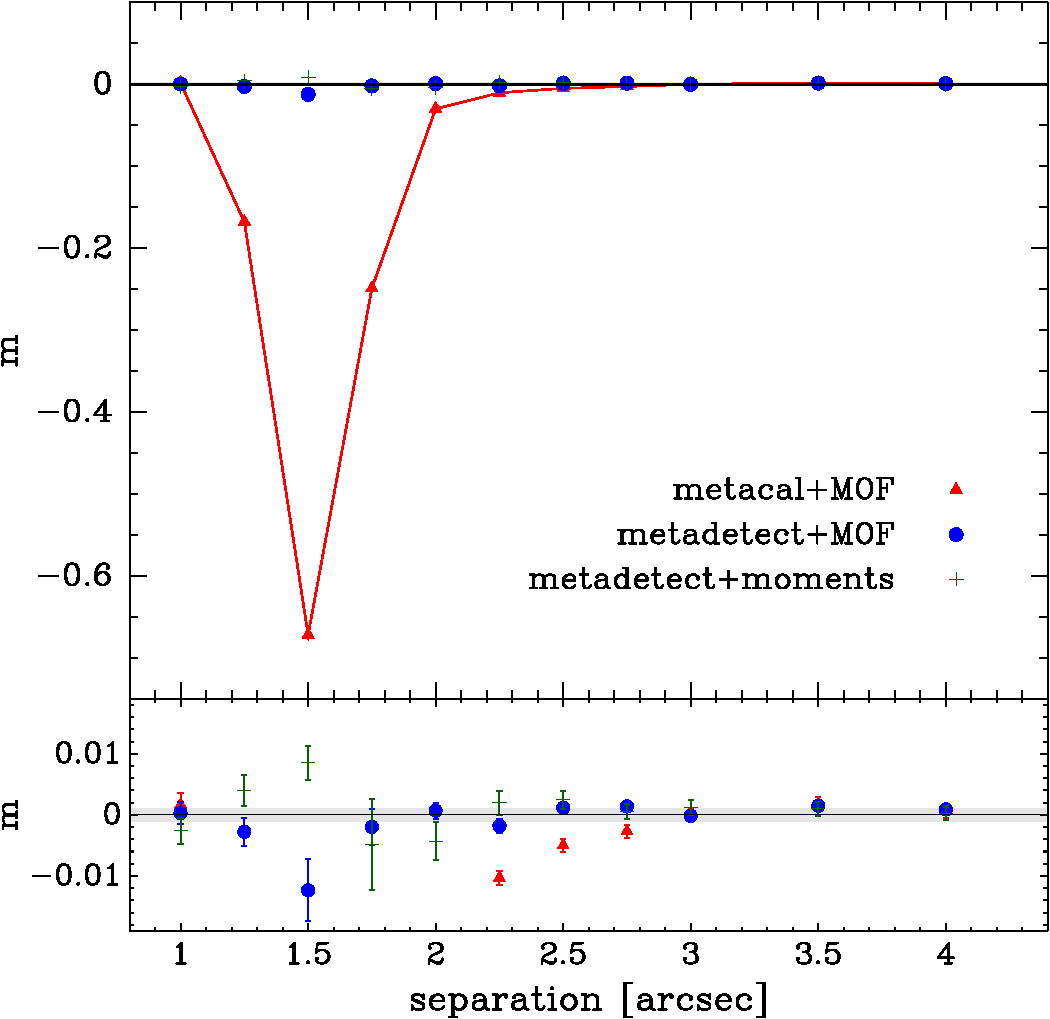
\includegraphics[width=\columnwidth]{pairs-mc-bdkpair.pdf}

\end{figure}
Erin's pair tests

\subsection{Bias in Simulations with Representative Galaxy Density and Noise}

Erin's tests with WeakLensingDeblending and Matt's tests

\begin{table}
    \centering
    \begin{tabular}{|l|l|c|c|}
        \hline
        Sim & Method         & \snr\ Cut & m             \\
        \hline
        \hline
        DES & MOF+metacal    & \snr$ > 10$ & $-0.016 \pm 0.003$  \\
        DES & MOF+metacal    & \snr$ > 15$ & $-0.038 \pm 0.003$  \\
        DES & MOF+metacal    & \snr$ > 20$ & $-0.053 \pm 0.003$  \\
        \hline
        LSST  & MOF+metacal    & \snr$ > 10$ & $-0.131 \pm 0.005$  \\
        LSST  & MOF+metacal    & \snr$ > 15$ & $-0.124 \pm 0.005$  \\
        LSST  & MOF+metacal    & \snr$ > 20$ & $-0.149 \pm 0.005$  \\
        \hline


    \end{tabular}
    
    \caption{
            Bias for standard \mcal\ with MOF deblending in simulations with
            realistic galaxy size, flux and noise.  In all cases a cut of
            $T/T_{PSF} > 0.5$ was also applied.  \ess{numbers are placeholders,
            need to run regular MOF+metacal on descwl sims}
            \label{tab:mcal:deblending}
    }

\end{table}


\section{Mitigating Shear-dependent Detection Biases with \textsc{METACALIBRATION}}
blah

\subsection{Results for Simulated Galaxy Pairs}

Erin's results with pairs.  Discuss results in the figure.

\subsection{Results for Simulations with Representative Galaxy Density and Noise}
\label{sec:res:constpsf}

Erin's results with WeakLensingDeblending and Matt's tests without
psf variation or masking

\begin{table}
    \centering
    \begin{tabular}{|l|l|c|c|}
        \hline
        Sim & Method         & \snr\ Cut & m             \\
        \hline
        \hline
        DES & \mdet+moments & \snr$ > 10$ & $-0.0010 \pm 0.0013$  \\
        DES & \mdet+moments & \snr$ > 15$ & $+0.0000 \pm 0.0013$  \\
        DES & \mdet+moments & \snr$ > 20$ & $+0.0002 \pm 0.0013$  \\
        \hline
        LSST  & \mdet+moments & \snr$ > 10$ & $-0.0027 \pm 0.0011$  \\
        LSST  & \mdet+moments & \snr$ > 15$ & $-0.0018 \pm 0.0011$  \\
        LSST  & \mdet+moments & \snr$ > 20$ & $+0.0001 \pm 0.0011$  \\
        \hline


    \end{tabular}
    
    \caption{
        Bias for \mcal, including detection in the process (a.k.a. \mdet).  These
        simulations have no PSF variation or masking.  No
        deblending was performed, and simple weighted moments were used
        without PSF correction.  In all cases a cut of $T/T_{PSF} > 0.5$ was
        also applied.  \ess{LSST needs to be redone with better
        psf handling.  } \label{tab:mdet:constpsf}
    }

\end{table}



\subsection{Results for Simulations with Realistic Masking and PSF Variation}
\label{sec:res:varpsf}

Matt's stuff with the full glory.  If all are equally unbiased, we can remove
secion \ref{sec:res:constpsf}

\begin{table}
    \centering
    \begin{tabular}{|l|l|c|c|}
        \hline
        Sim & Method         & \snr\ Cut & m             \\
        \hline
        \hline
        DES & \mdet+moments & \snr$ > 10$ & $-0.0010 \pm 0.0013$  \\
        DES & \mdet+moments & \snr$ > 15$ & $+0.0000 \pm 0.0013$  \\
        DES & \mdet+moments & \snr$ > 20$ & $+0.0002 \pm 0.0013$  \\
        \hline
        LSST  & \mdet+moments & \snr$ > 10$ & $-0.0027 \pm 0.0011$  \\
        LSST  & \mdet+moments & \snr$ > 15$ & $-0.0018 \pm 0.0011$  \\
        LSST  & \mdet+moments & \snr$ > 20$ & $+0.0001 \pm 0.0011$  \\
        \hline


    \end{tabular}
    
    \caption{
        Same as table \ref{tab:mdet:constpsf} but with realistic masking and
        spatial PSF variation.  \ess{numbers are placeholders} \label{tab:mdet:varpsf}
    }

\end{table}


\section{Summary}
blah

\bibliographystyle{mnras}
\bibliography{references}

\end{document}
